\documentclass[10pt]{article}

\usepackage{fixme}
\fxsetup{ status=draft, layout=inline}
\usepackage[pdftex]{graphicx}

\ExecuteOptions{letterpaper,10pt,twocolumn,oneside,final,journal}

\begin{document}

\section{Introduction}

Monitoring the meteorology and vegetation phenomenon is the cornerstone and challenge of ecology and biology research. Expensive satellite images give large scale data but struggle with cloud cover, 
atmospheric conditions and fine-grained localization such as flower species distribution, human interaction with nature,
% and direct targeting of them, 
% \cite{China tests anti-satellite weapon, unnerving U.S., Pentagon is confident missile hit satellite tank}
% need new or more deficiency of satellites
while citizen science provides high quality data but is also costly and is very difficult to practice over large scale areas.
The enormous popularity of photo-sharing website collects images in large spatial scale, from under clouds and in close focus (compare to aerial surveillance), 
moreover, they are freely accessible to the public.
The more than 300 million images uploaded to social media every day
\cite{https://zephoria.com/top-15-valuable-facebook-statistics/}
 potentially contain not only human activities, but also outdoor ecology and biology information intentionally and incidentally as shown in Figure \ref{fig:flickrexp}.
% !! extend

The idea of reproducing satellite maps has become more and more interesting to scientists applying textual mining on \fxnote{cite{stock, ecology, election, tourists}}, 
and recently to computer vision researches directly deriving \fxnote{cite{temperature, cloud, mountain peak}} information from visual content.
In this paper, we test the feasibility of leveraging these noisy and biased images as a new approach to observe nature. We study 2 particular phenomena, snowfall and vegetation coverage as they are fundamental topic in ecology and biology study, have relatively distinct appearance to recognize, have a good chance to appear in social media, and also have satellite maps available to serve as ground truth. Our approach is illustrated in Figure \ref{fig:overview}. 
% new source of monitoring ecology information
First, we collect a large hand-labeled data set of the existence or absence of ecology phenomena. 
Then, we train a classifier for each phenomenon by combining its most discriminative visual features and by using deep learning features. 
Finally, we collect 12 million images from entire North America over 2 years, make prediction on geo and temporal scale by aggregating this visual evidence.

This paper is built on our earlier work \fxnote{cite{www}} analyzing ecology phenomenon from image tags only. We apply a new approach understanding visual content of images, and run experiments on the exact same data set to study how vision techniques could help in social media data mining compared to using textual data alone. Also, to our best knowledge, among all the research works performing social sensing with image data, this is the first one providing continental scale quantitative performance evaluation.


\begin{figure*}[h]
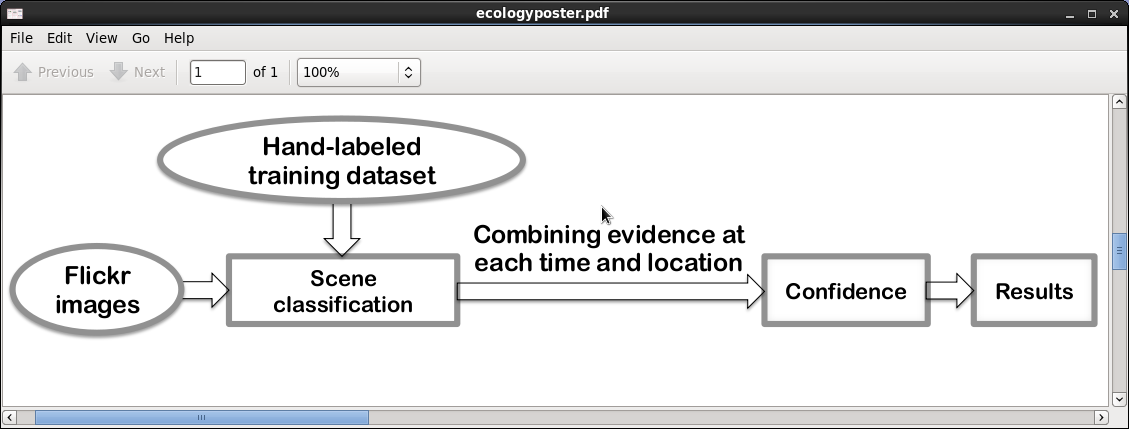
\includegraphics[scale=.3]{figure/overview.png}
\caption{Overview of our approach to apply image classifiers on large scale images and make prediction by aggregating these visual evidence. \fxnote{first classifier, then prediction}}
\label{fig:overview}
\end{figure*}


\begin{figure*}[th]
{\small{
\begin{center}
\begin{tabular}{@{}c@{\,\,\,}c@{\,\,\,}c@{\,\,\,}c@{\,\,\,}}
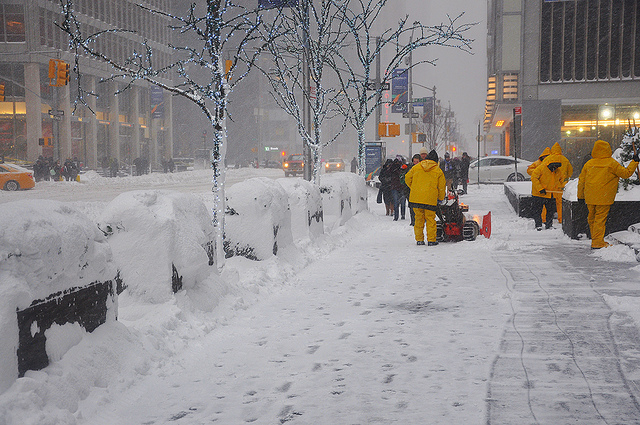
\includegraphics[width=0.19\textwidth, height=0.7in]{image/citysnow.jpg} &
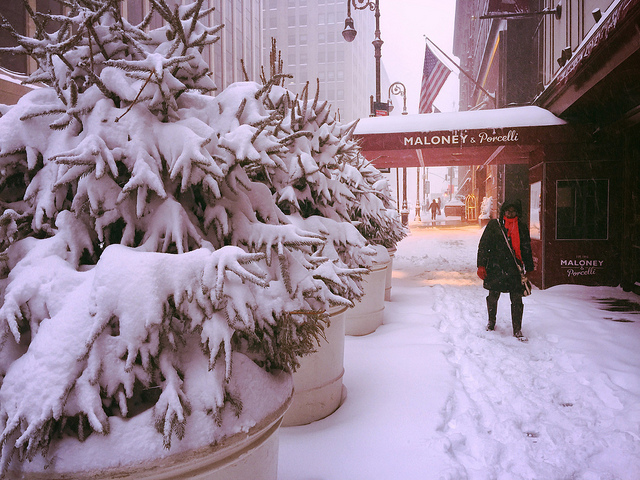
\includegraphics[width=0.19\textwidth, height=0.7in]{image/citysnow2.jpg} &
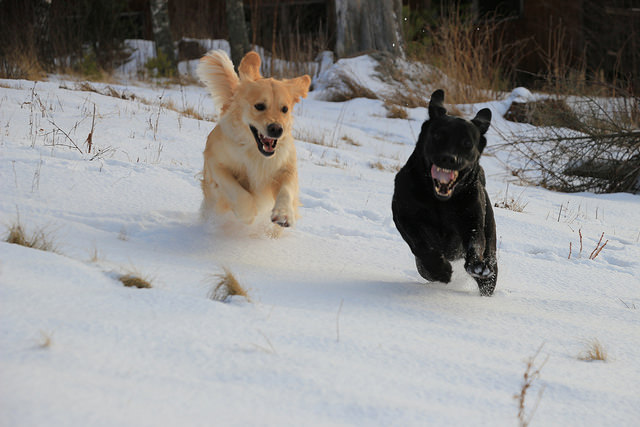
\includegraphics[width=0.19\textwidth, height=0.7in]{image/dogsnow.jpg} &
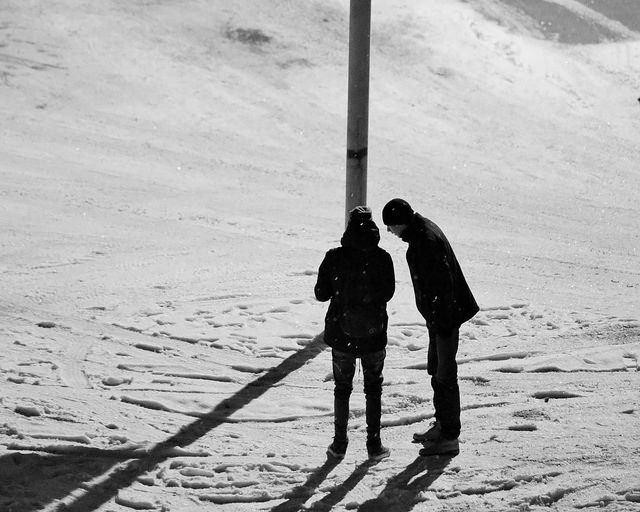
\includegraphics[width=0.19\textwidth, height=0.7in]{image/humansnow.jpg} \\
%\multicolumn{5}{c}{(a) Random positive images in vegetation dataset} \\ 
\\[-6pt]
\hline
\\[-6pt]
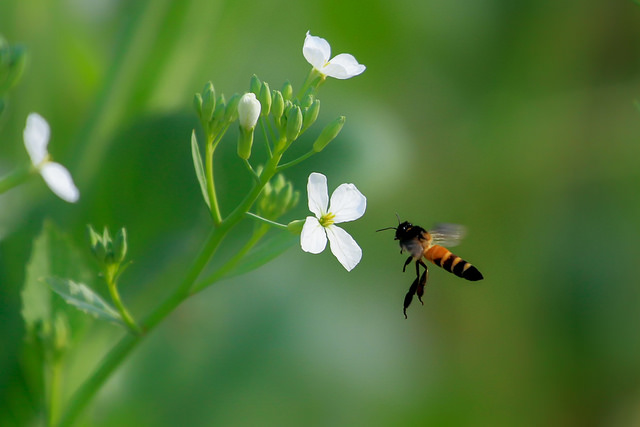
\includegraphics[width=0.19\textwidth, height=0.7in]{image/intentiongreen.jpg} &
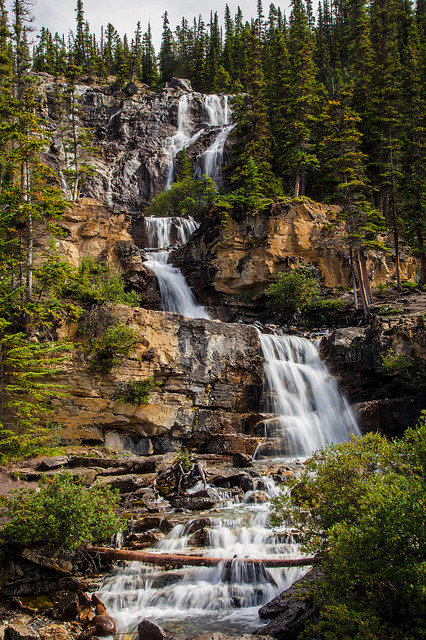
\includegraphics[width=0.19\textwidth, height=0.7in]{image/waterfallgreen.jpg} &
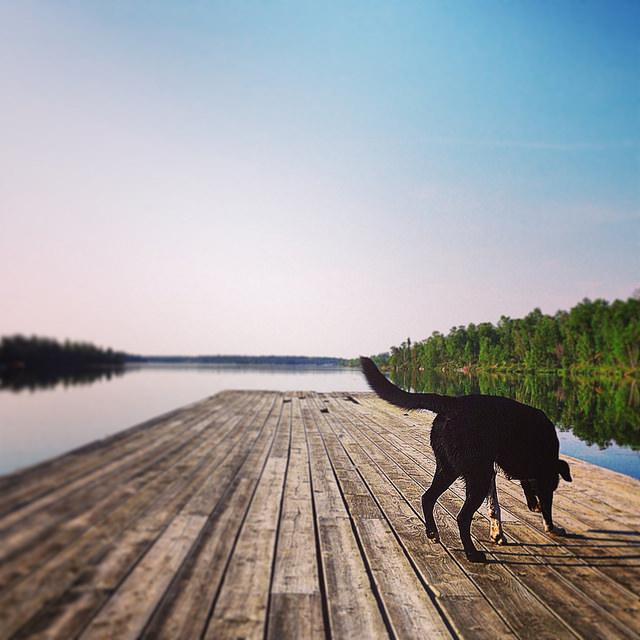
\includegraphics[width=0.19\textwidth, height=0.7in]{image/dogtree.jpg} &
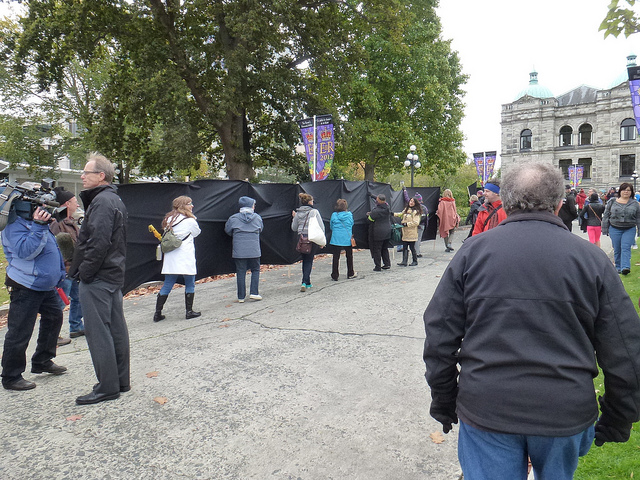
\includegraphics[width=0.19\textwidth, height=0.7in]{image/humantree.jpg} \\
%\multicolumn{5}{c}{(b) Random negative images in vegetation dataset} \\
\end{tabular}
\end{center}
}}
\caption{Flickr image examples capture snow and greenery evidence on purpose and as background.}
\label{fig:flickrexp}
\end{figure*}

\end{document}
